\documentclass[xcolor=table]{beamer}

\usetheme{Boadilla}
\usecolortheme{dolphin}
\useoutertheme[subsection=false]{smoothbars}

\setbeamercolor{frametitle}{fg = black, bg = white} 
\setbeamercolor{palette primary}{use=structure,fg=white,bg=structure.fg!60!white}
\setbeamercolor{palette secondary}{use=structure,fg=white,bg=structure.fg!90!white}
\setbeamercolor{palette tertiary}{use=structure,fg=white,bg=structure.fg!120!white}
\setbeamercolor{palette quaternary}{use=structure,fg=black,bg=white} %Top bar

\setbeamertemplate{enumerate subitem}[circle]%
\renewcommand{\insertsubenumlabel}{\alph{enumii}}

\usepackage{amsmath}
\usepackage{xcolor}
\usepackage{booktabs}
\usepackage[utf8]{inputenc}
\usepackage{hyperref}
\usepackage[table]{xcolor}
\definecolor{lightgray}{gray}{0.9}

\hypersetup{
    colorlinks,
    citecolor=blue,
    linkcolor=blue
}

\footnotesize \let\small\footnotesize

\author{Jonathan P. Latner, PhD}
\title{Tuning GANs}
\date{\today}

\beamertemplatenavigationsymbolsempty 
\setbeamerfont{page number in head/foot}{size=\tiny}
\setbeamertemplate{footline}[frame number]
\setbeamertemplate{caption}[numbered]
\setbeamertemplate{section in toc}[sections numbered]

\begin{document}



% \section{Introduction}\label{sec:intro}
\frame{\frametitle{ }
\titlepage
\thispagestyle{empty}
}

% \frame{\frametitle{}
% \begin{table}[!h]
%     \caption{Sample selection steps}
%     \centering
%     \resizebox{.9\textwidth}{!}{\input{../../tables/descriptives_table_steps_presentation.tex}}
%     \label{descriptives_table_steps}
% \end{table}
% }

\frame{\frametitle{Tuning CTGAN}
\begin{itemize}
    \item Batch size (constant steps)
    \item Epochs (constant batch size)
    \item Dimensions (2 hyperparameters)
    \begin{itemize}
        \item embedding\_dim (int): Size of the random sample passed to the Generator. Defaults to 128.
        \item dimensionality - 2 hyperparameters, but same value for each
        \begin{itemize}
            \item discriminator\_dim (tuple or list of ints): Size of the output samples for each one of the Discriminator Layers. A Linear Layer will be created for each one of the values provided. Defaults to (256, 256).
            \item generator\_dim (tuple or list of ints): Size of the output samples for each one of the Residuals. A Resiudal Layer will be created for each one of the values provided. Defaults to (256, 256).  
        \end{itemize}
    \end{itemize}
\end{itemize}
}

\frame{\frametitle{Batch size, epochs, and steps}
\begin{table}[!h]
    \rowcolors{1}{white}{lightgray}
    \caption{}
    \centering
    \begin{tabular}{cllll}
    \toprule
    N & Batch size & Steps per Epoch & Epochs & Actual Steps \\
    \midrule
    5.000 & 100 & 50 & 60 & 3,000 \\
    5.000 & 250 & 20 & 150 & 3,000 \\
    5.000 & 500 & 10 & 300 & 3,000 \\
    5.000 & 1.000 & 5 & 600 & 3,000 \\ \hline
    5.000 & 500 & 10 & 100 & 1,000 \\
    5.000 & 500 & 10 & 300 & 3,000 \\
    5.000 & 500 & 10 & 600 & 6,000 \\
    5.000 & 500 & 10 & 900 & 9,000 \\
    \bottomrule
    \end{tabular}
\end{table}
}



% \section{Results}\label{sec:results}
\frame{\frametitle{Effect of batch size (constant steps)}
\begin{figure}
    \caption{}
    \resizebox{.75\textwidth}{!}{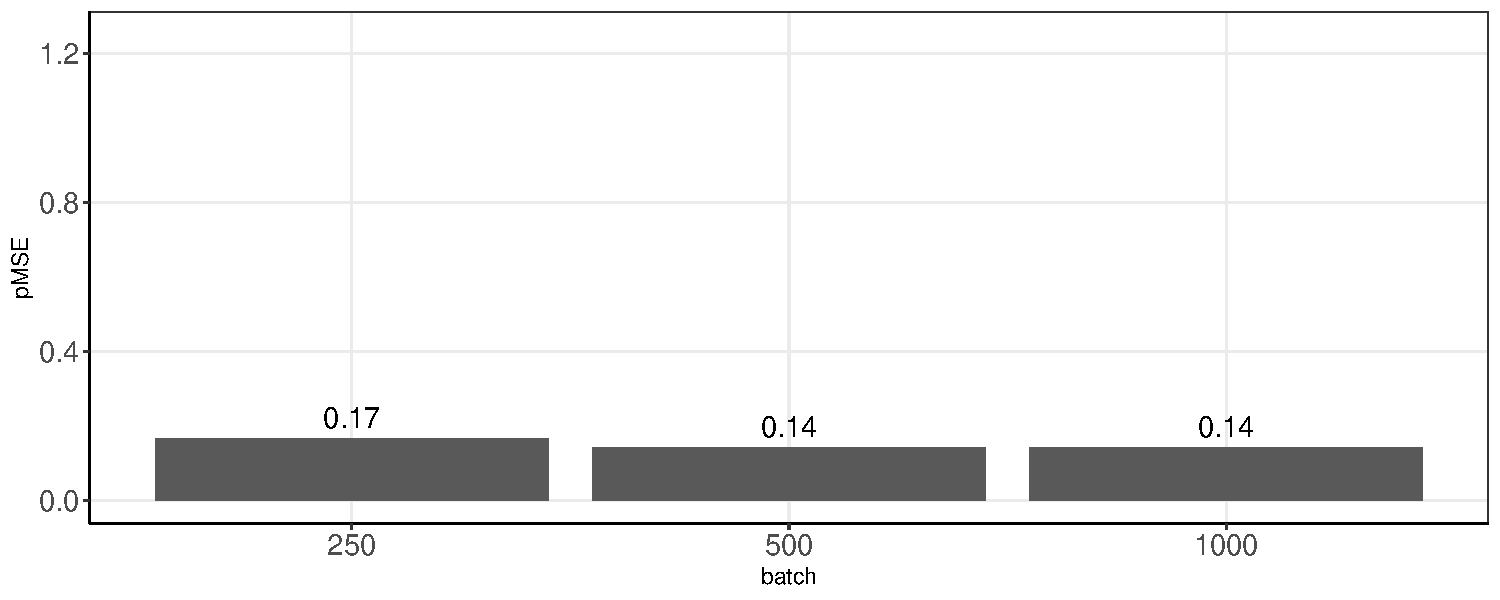
\includegraphics{../graphs/ctgan/ctgan_fidelity_optimize_batch_size.pdf}}
    \label{ctgan_fidelity_optimize_batch_size}
\end{figure}
}

\frame{\frametitle{Effect of epochs (constant batch size)}
\begin{figure}
    \caption{}
    \resizebox{.75\textwidth}{!}{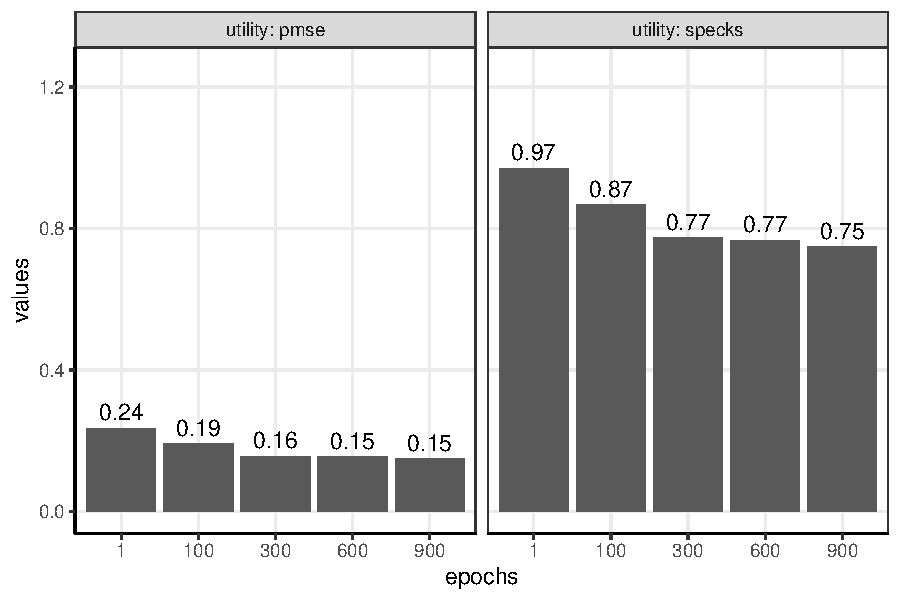
\includegraphics{../graphs/ctgan/ctgan_fidelity_optimize_epochs.pdf}}
    \label{ctgan_fidelity_optimize_epochs}
\end{figure}
}

\frame{\frametitle{Effect of dimensions}
\begin{figure}
    \caption{}
    \resizebox{.8\textwidth}{!}{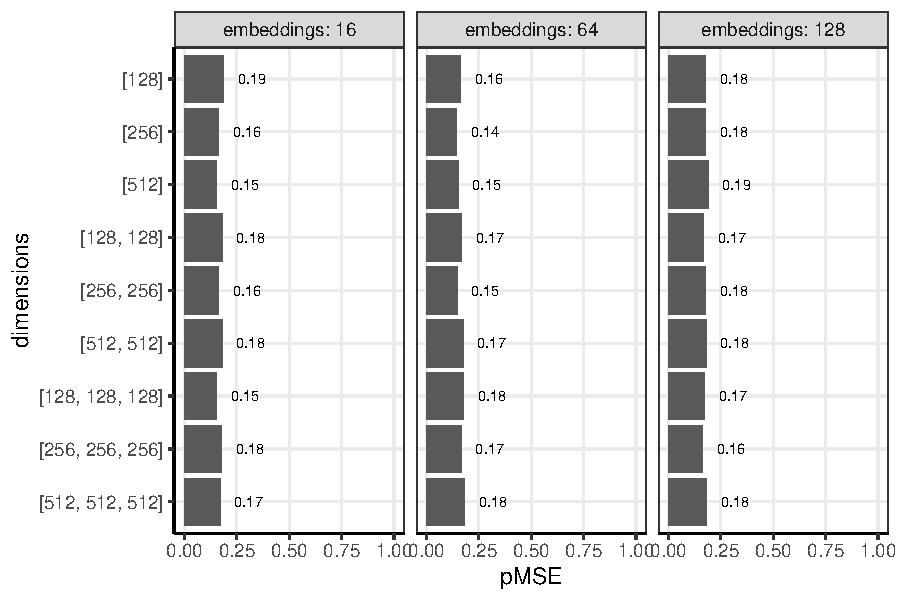
\includegraphics{../graphs/ctgan/ctgan_fidelity_optimize_dimensions.pdf}}
    \label{ctgan_fidelity_optimize_dimensions}
\end{figure}
}

\frame[c]{\frametitle{}
\centering
Thank you\\\

}


\end{document}


